%%%%%%%%%%%%%%%%%%%%%%%%%%%%%%%%%%%%%%%%%%%%%%%%%%%%%%%%%%%%%%%%%%%%
%% chapter3.tex
%% UNL thesis document file
%%
%% Chapter with a short laext tutorial and examples
%%%%%%%%%%%%%%%%%%%%%%%%%%%%%%%%%%%%%%%%%%%%%%%%%%%%%%%%%%%%%%%%%%%%
\chapter{State Of the Art}
\label{cha:stateofart}


\section{Multimodal Machine Learning}

Information is being exchanged through different channels. These different channels can be called modalities. The same way humans can process information coming from different sources in order to take conclusions and take action, the ultimate goal of artificial intelligence is to understand the world around us by collecting, interpreting and reasoning multimodal data. This field can be called \textbf{Multimodal Machine Learning} which aims to build models that can process and relate information from multiple modalities and which is gaining more and more importance and has extraordinary potential \cite{Baltruvsaitis2017multimodal}.

Although Multimodal Machine Learning brings many challenges given the heterogeneity of data, the hope is to gain a deeper understanding of natural phenomena as data from multimodal sources are used to capture correspondences between the modalities.

One of the first examples of multimodal research is audio-visual speech recognition (AVSR) in 1989. The motivation came from the discovered McGurk effect in which it was found that human perception of sound is not independent from the visual perception. During the experiment subjects heard the syllable /ba-ba/ while they the lips of a person saying /ga-ga/, however, they perceived the sound /da-da/. Researcher from the speech community started to include visual information in their investigations. Although research in AVSR is not common currently, the deep learning community showed renewd interest \cite{Ngiam2011}. What was shown in the experiental results in AVSR is that the captured interactions between speech and visual information were not complementary but rather supplementary. For ex. experimental results showed more advantage of using visual information when the speech signal was noisy but not when the scenario was noiseless.
In \cite{Dmello2015review} several multimodal affect recognition results were compared and their meta-analysis revealed that a majority of recent work on multimodal affect recognition showed an improvement when using more than one modality. However, the improvement on naturally-occurring emotions is reduced. 

There are main challenges (taken from \cite{Baltruvsaitis2017multimodal}, \todo{rephrase}):
\begin{enumerate}
\item \textbf{Representation:} A first fundamental challenge is learning how to represent and summarize multimodal data in a way that exploits the complementarity and redundancy of multiple modalities. The heterogeneity of multimodal data makes it challenging to construct such representations. For example, language is often symbolic while audio and visual modalities will be represented as signals.
\item \textbf{Translation:} A second challenge addresses how to translate (map) data from one modality to another. Not only is the data heterogeneous, but the relationship between modalities is often open-ended or subjective. For example, there exist a number of correct ways to describe an image and and one perfect translation may not exist.
\item \textbf{Alignment:} A third challenge is to identify the direct relations between (sub)elements from two or more different modalities. For example, we may want to align the steps in a recipe to a video showing the dish being made. To tackle this challenge we need to measure similarity between different modalities and deal with possible longrange dependencies and ambiguities.
\item \textbf{Fusion:} A fourth challenge is to join information from two or more modalities to perform a prediction. For example, for audio-visual speech recognition, the visual description of the lip motion is fused with the speech signal to predict spoken words. The information coming
from different modalities may have varying predictive power and noise topology, with possibly missing data in at least one of the modalities.
\item \textbf{Co-learning:} A fifth challenge is to transfer knowledge between modalities, their representation, and their predictive models. This is exemplified by algorithms of cotraining,
conceptual grounding, and zero shot learning.
Co-learning explores how knowledge learning from one modality can help a computational model trained on a different modality. This challenge is particularly relevant when one of the modalities has limited resources (e.g., annotated data).
\end{enumerate}

\subsection{Multimodal Representations}
\todo{rephrase}
Following the work of Bengio et al. [17]
we use the term feature and representation interchangeably, with each referring to a vector or tensor representation of an entity, be it an image, audio sample, individual word, or a sentence. A multimodal representation is a representation of data using information from multiple such entities. \cite{Baltruvsaitis2017multimodal}


There are different challenges when it comes to represent multimodal data: how to combine data from heterogeneous soures; how to deal with different levels of noise; and how to deal with missing data. \cite{Baltruvsaitis2017multimodal}

\textbf{Backbone of any multimodal model is the representation of the data!} Good representations are important for the performance of machine learning models.

In \cite{Bengio2013representation} the characteristics of good representations are listed: smoothness, temporal and spatial coherence, sparsity, and natural clustering amongst others. In \cite{Srivastava2012} additional desirable properties for multimodal represenations are listed such as similarity in the representation space should reflect similarity of the corresponding concepts, the representation should be easy to obtain even in the absence of some modalities, and it should be possible to fill-in missing modalities given observed ones.

Unimodal representations have been studied extensively in the past and recently a shift has been observed from hand-designed representations (e.g. SIFT) for specific applications to data-driven using f.ex. convolutional neural networks (CNN). Until recently multimodal representations involved simple concatenation of unimodal ones but this has been changing rapidly.\cite{Baltruvsaitis2017multimodal}

According to \cite{Baltruvsaitis2017multimodal} there are two types of multimodal representation: joint and coordinated. 
\subsubsection{Joint representations} combine unimodal signals into the same representation space:
$x_m = f(x_1, \cdots, x_n),$
multimodal representaion $x_m$ is computed using function $f$ using f.ex. a deep neural network, restricted Boltzmann machine, or a recurrent neural network that relies on unimodal representations $x_1,\cdots, x_n $. 
Joint representations are mostly used in tasts where multimodal data is present during traininf and inference steps. One xample is early fusion which is the simple concatenation of individual modality features. More advanced methods are neural networks, graphical models and recurrent neural networks.

\textbf{Neural networks} are very popular for unimodal representation such as visual, acoustic, and textual data, and are increasingly used in the mutimodal domain.
In general, neural networks are made up of successive building blocks of inner products followed by non-linear activation functions. In order to use a neural network as a way to represent data, it is first trained to perform a specific task (e.g., recognizing objects in images). Due to the multilayer nature of deep neural networks each successive layer is hypothesized to represent the data in a more abstract way [17], hence it is common to use the final or penultimate neural layers as a form of data representation. To construct a multimodal representation using neural networks each modality starts with several individual neural layers followed by a hidden layer that projects the modalities into a joint space [9], [145], [156], [227]. The joint multimodal representation is then be passed through multiple hidden layers itself or used directly for prediction. Such models can be trained end-to-end — learning both to represent the data and to perform a particular task.
This results in a close relationship between multimodal representation learning and multimodal fusion when using neural networks.
The major advantage of neural network based joint representations
comes from their often superior performance
and the ability to pre-train the representations in an unsupervised
manner. The performance gain is, however, dependent on the amount of data available for training. One of the disadvantages comes from the model not being able to handle missing data naturally — although there are ways to alleviate this issue [151], [217]. Finally, deep networks are often difficult to train [69], but the field is making progress in better training techniques

\textbf{Probabilistic graphical models} construct representations using latent random variables. Popular approaches are deep Boltzmann machines (DBM) which stack restricted Boltzmann machines (RBM) as building blocks. Similar to neural networks, each layer represents the data at a higher level of abstraction. The advantage is that DBM do not need supervised data for training. These graphical models represten the data in a probabilistic manner, but it can be converted to deterministic neural networks with the cost of loosing the generative aspect of the model which allows to deal with missing data even if a whole modality is missing.
\textcolor{red}{Multimodal deep belief networks } have been extended to multimodal DBMs which are able to learn joint representations from multiple modalities by merging two or more undirected graphs using a binary layer of hidden units on top of them. They allow for the low level representations of each modality to influence each other after the joint training due to the undirected nature of the model. Similar to autoencoders
the representation can be trained in an unsupervised manner enabling the use of unlabeled data. The major disadvantage of DBMs is the difficulty of training them — high computational cost, and the need to use approximate variational training methods.

\textbf{Sequential Representation} is used for data with varying length sequences such asentences, videos, or audio streams. Recurrent neural networs (RNNs) and their variants such as long-short term memory \textcolor{red}{(LSTMs)} networks have been used with success in sequence modeling across various tasks. RNNS have been used ro represent various unimodal signals such as sequences of words, audio, or images, with most succes in the language domain. Similar to traditional neural networks, the hidden state of an RNN can be seen as a representation of the data, i.e., the hidden state of RNN at timestep $t$
can be seen as the summarization of the sequence up to that timestep.

Joint representations project multimodal data into a common space and are best suited for situations when all of the modalities are present during inference. They have been extensively used for AVSR, affect, and multimodal gesture recognition.
 
\subsubsection{Coordinated representations} process unimodal signals separately, but enforce certain similarity constraints on them to bring them to what we term a coordinated space.
$f(x_1) \sim g(x_2)$,
where each modality has a corresponding projection function ($f$ and $g$ above) that maps it into a coordinated multimodal space.
the projection into the multimodal space is independent for each modality, but the resulting space is coordinated between them (indicated as $\sim$). Examples are minimizing cosine distance, maximizing correlation, and enforcing a partial order between the resulting spaces.

There are coordinated representations that enforce similarity between representations and coordinated representations that enforce \textcolor{red}{more structure} on the resulting space. The first ones, \textbf{similarity models} minimize the distance between modalities in the coordinated space. WSABIE model was one of the earliest examples where a coordinated space was constructed for images and their annotations using a linear mapping from image and textual features such that the corresponding annotation and image representation would have a higher inner product (smaller cosine distance).

Neural networks have become popoular to construct coordinated represenetations as they can jointly learn coordinated representations in an end-to-end manner. An example is DeViSE- a deep visual-semantic embedding.It uses a similar inner product and ranking loss function to WSABIE but uses more complex image and word embeddings. 
Kiros et al. [105] extended this to
sentence and image coordinated representation by using an LSTM model and a pairwise ranking loss to coordinate the
feature space. Socher et al. [191] tackle the same task, but extend the language model to a dependency tree RNN to incorporate compositional semantics. A similar model was
also proposed by Pan et al. [159], but using videos instead of images. Xu et al. [231] also constructed a coordinated space between videos and sentences using a hsubject, verb,
objecti compositional language model and a deep video model. This representation was then used for the task of cross-modal retrieval and video description.




\subsection{Application}
\subsubsection{Audio-Visual Speech Recognition}


\subsubsection{Lip-Reading}

\subsubsection{Affective Computing}

\cite{Narayanan2013} Behavioral signal processing: \\
from \url{http://people.csail.mit.edu/jrg/meetings/2016-Feb8-ShriN.pdf}\\
\begin{itemize}
    \item computing behavioral traits \& states for decision making and action
    \item help do things we know to do well more efficiently, consistently
    \item help handle new data, create new models to offer unimagined insights: create tools for discovery
    \item FOCUS OF THE TALK ON SPEECH AND SPOKEN LANGUAGE CUES
    \item HEALTH \& WELL BEING APPLICATIONS
\end{itemize}

see graph with applications domains\\
combination of vocal, language, and visual behavioral cues\\
ex. see uncertainty vs certainty\\
frequent application: 
\begin{itemize}
    \item marital therapy $\rightarrow$ characterizing affective dynamics, humor, blame patterns
    \item Autism spectrum disorders $\rightarrow$ technologies for rich understanding of expressive behavior and interaction
\end{itemize}

Multimodal behavior signals:\\
\begin{itemize}
    \item Provide a window into internal state \& processes $\rightarrow$ Some overly expressed and directly observable (e.g., vocal and facial expressions, body posture)
$\rightarrow$ Others, covert
(e.g., heart rate, electrodermal response, brain activity) 
    \item Implications for understanding $\rightarrow$ Human information encoding and decoding $\rightarrow$ “Mind-Body” relations
$\rightarrow$ People’s judgment of others behavior
    \item MEASURING \& QUANTIFYING HUMAN BEHAVIOR: A CHALLENGING ENGINEERING PROBLEM
\end{itemize}


\section{Available Datasets}

\textbf{SEMAINE Database: }
conversation with a virtual agent; study interpersonal dynamics between
speakers and listeners. This dataset was used for the fisr audio-visual emotion challenge (AVEC) in 2011. \url{https://semaine-db.eu}\\

\textbf{SEWA Database: }
The SEWA database includes annotations of the recordings in terms of facial landmarks, facial action unit (FAU) intensities, various vocalisations, verbal cues, mirroring, and rapport, continuously valued valence, arousal, liking, and prototypic examples (templates) of (dis)liking and sentiment. The data has been annotated in an iterative fashion, starting with a sufficient amount of examples to be annotated in a semi-automated manner and used to train various feature extraction algorithms developed in SEWA, and ending with a large DB of annotated facial behaviour recorded in the wild. Used for AVEC 2017. \url{https://db.sewaproject.eu}\\

\textbf{HUMAINE Database:} 
This is a the HUMAINE database which became available at the end of 2007. It consists of an exemplar set of 50 clips from naturalistic and induced data showing a range of modalities and emotions, and a subset of 16 clips selected to cover a balanced sample of emotional behaviour in a range of contexts. This subset is labelled. \url{http://humaine-db.sspnet.eu/}\\

\textbf{EATMINT database: }
The EATMINT database contains multi-modal and multi-user recordings of affect and social behaviors in a collaborative setting. The following signals were recorded for 30 dyads (i.e. 60 participants) :
\begin{itemize}
\item Physiological signals: electrocardiogram, electrodermal activity (GSR), blood volume pulse, respiration and skin temperature;
\item Behaviors: eye-movements (eye-tracking), facial expressions, software actions logs;
\item Discourse: speech signals and transcripts.
\end{itemize}
Each interaction is annotated in term of affect, collaboration and social aspects (e.g. conflict, grounding, etc.) \url{https://eatmint.unige.ch/home.php}\\

\textbf{RECOLA multimodal database:} The database consists of 9.5 hours of audio, visual, and physiological (electrocardiogram, and electrodermal activity) recordings of online dyadic interactions between 46 French speaking participants, who were solving a task in collaboration. Affective and social behaviors expressed by the participants were reported by themselves, at different steps of the study, and by six French-speaking assistants using the ANNEMO web-based annotation tool (time and value 'continuous'), for the first five minutes of interaction; 3.8 / 2.9 hours of annotated audiovisual / multimodal data, respectively. \url{https://diuf.unifr.ch/diva/recola/}\\

\textbf{MMDB:} We introduce the Multimodal Dyadic Behavior (MMDB) dataset, a unique collection of multimodal (video, audio, and physiological) recordings of the social and communicative behavior of toddlers. The MMDB contains 160 sessions of 3-5 minute semi-structured play interaction between a trained adult examiner and a child between the age of 15 and 30 months. Our play protocol is designed to elicit social attention, back-and-forth interaction, and non-verbal communication from the child. These behaviors reflect key socio-communicative milestones which are implicated in autism spectrum disorders. The MMDB dataset supports a novel problem domain for activity recognition, which consists of the decoding of dyadic social interactions between adults and children in a developmental context. \url{http://www.cbi.gatech.edu/mmdb/}

\textbf{EmoReact:} A newly collected multimodal emotion dataset of children between the ages of four and fourteen years old that contains 1102 videos; the biggest dataset of its kind. These videos are annotated for 17 affective states, including six basic emotions (happiness, sadness, surprise, fear, disgust, and anger), neutral, valence and nine complex emotions including curiosity, uncertainty, excitement, attentiveness, exploration, confusion, anxiety, embarrassment and frustration. We provide a detailed analysis of the visual and vocal behaviors shown by children expressing these emotions.
\section{Available APIs for face analysis}

\textbf{Healthcare:} 
Quote: "We use facial analysis, deep learning and artificial intelligence to transform big data into actionable genomic intelligence to improve diagnostics and therapeutics. With the world’s largest network of clinicians, labs and researchers creating one of the fastest growing and most comprehensive genomic databases, FDNA is changing the game for rare disease patients."
\url{http://www.fdna.com}\\


\textbf{OpenFace:}
Quote:OpenFace is a Python and Torch implementation of face recognition with deep neural networks and is based on the CVPR 2015 paper FaceNet: A Unified Embedding for Face Recognition and Clustering by Florian Schroff, Dmitry Kalenichenko, and James Philbin at Google. Torch allows the network to be executed on a CPU or with CUDA. Freely available. \url{https://cmusatyalab.github.io/openface/}\\

\textbf{IMOTIONS:} combines Emotient face expression technology with other physiological signals such EEG, eye tracking, Galvanic Skin response, etc. to improve emotion recognition accuracy
\url{https://imotions.com/emotient/}\\

\textbf{EmoVu:} Deep learning based emotion recognition software that reads facial micro expressions. Uses CNNs, Challenging covariate factors such as pose and lighting variations are mitigated by employing robust face tracking, pose normalization and synthesis, and local lighting invariant feature descriptors. Misclassification is minimized through a rigorous classification scheme comprised of decision rule/filtering, classification, and verification stages. Our classifiers are trained on a large and diverse corpus of images to account for variations in appearance across different settings. Free trial available.
\url{http://emovu.com/e/developers/api/} \\

\textbf{Kairos:} "Provides an API for analyzing facial expressions and fea- tures for emotion recognition, gender and age detection and at- tention management. (Have key for free version)"\url{https://www.kairos.com}\\

\textbf{Project Oxford:} by Microsoft provides APIs for categories such as Vision, Speech, Language, Knowledge and Search. Can be tested for free.
\url{https://azure.microsoft.com/en-us/try/cognitive-services/}\\

\textbf{FaceReader:} by Noldus is widely used for academic purposes. It is a facial expression analysis software for analyzing universal emotions in addition to neutral and contempt. The software is also used to observe gaze direction and head orientation. Used more than 10,000 annotated images for training. Describes the face with 500 key points. Can be rented. 
\url{http://www.noldus.com/human-behavior-research/products/facereader}\\

\textbf{InSight} by Sightcorp is a facial expression analysis API and is also used for eye tracking, age and gender estimation, head pose estimation, etc. 2 weeks free trial.
\url{http://sightcorp.com/insight/}\\

Some papers

\begin{itemize}
    \item Learning to diagnose with LSTM recurrent neural networks
    \item Deep Patient: an unsupervised representation to predict the future of patients from the electronic health records
\end{itemize}





\section{Stuttering}
Questions from Stuttering Center Western Pennsylvania\\
- What makes a person stutter on a particular word or utterance?\\
- Which measures are most important when evaluating stuttering, and what is the most reliable way to obtain these measures?\\
- How do we document improvements in treatment when many of the changes are "under the surface" (e.g., changes in feelings or attitudes toward speaking)?\\
- How well does treatment work, and how does a clinician determine what type of treatment is best for a specific individual who stutters?\\
"Many current treatments for stuttering in school-age children, adolescents, and adults are based on finding a balance between helping speakers improve their fluency through changes to speech production ("speech modification" techniques) and helping speakers improve their attitudes and feelings about stuttering to reduce the severity of stuttering ("stuttering modification" techniques). Ultimately, the goal of treatment is to reduce the overall impact of stuttering on the person's life."\\




\section{Datasets}

List existing datasets and why the one I want to create is important! \url{http://vkc.mc.vanderbilt.edu/childhoodstuttering/forscientists_datasets.html}\\

paper: The UCLASS archive of stuttered speech\\


% \subsection{Inserting Figures Wrapped with text} % (fold)
% \label{ssec:inserting_images_wrapped_with_text}
% 
% You should only use this feature is \emph{really} necessary. This means, you have a very small image, that will look lonely just with text above and below.
% 
% In this case, you must use the \verb!wrapfiure! package.  To use \verb!wrapfig!, you must first add this to the preamble:
% 
% \begin{wrapfigure}{l}{2.5cm}
%   \centering
%     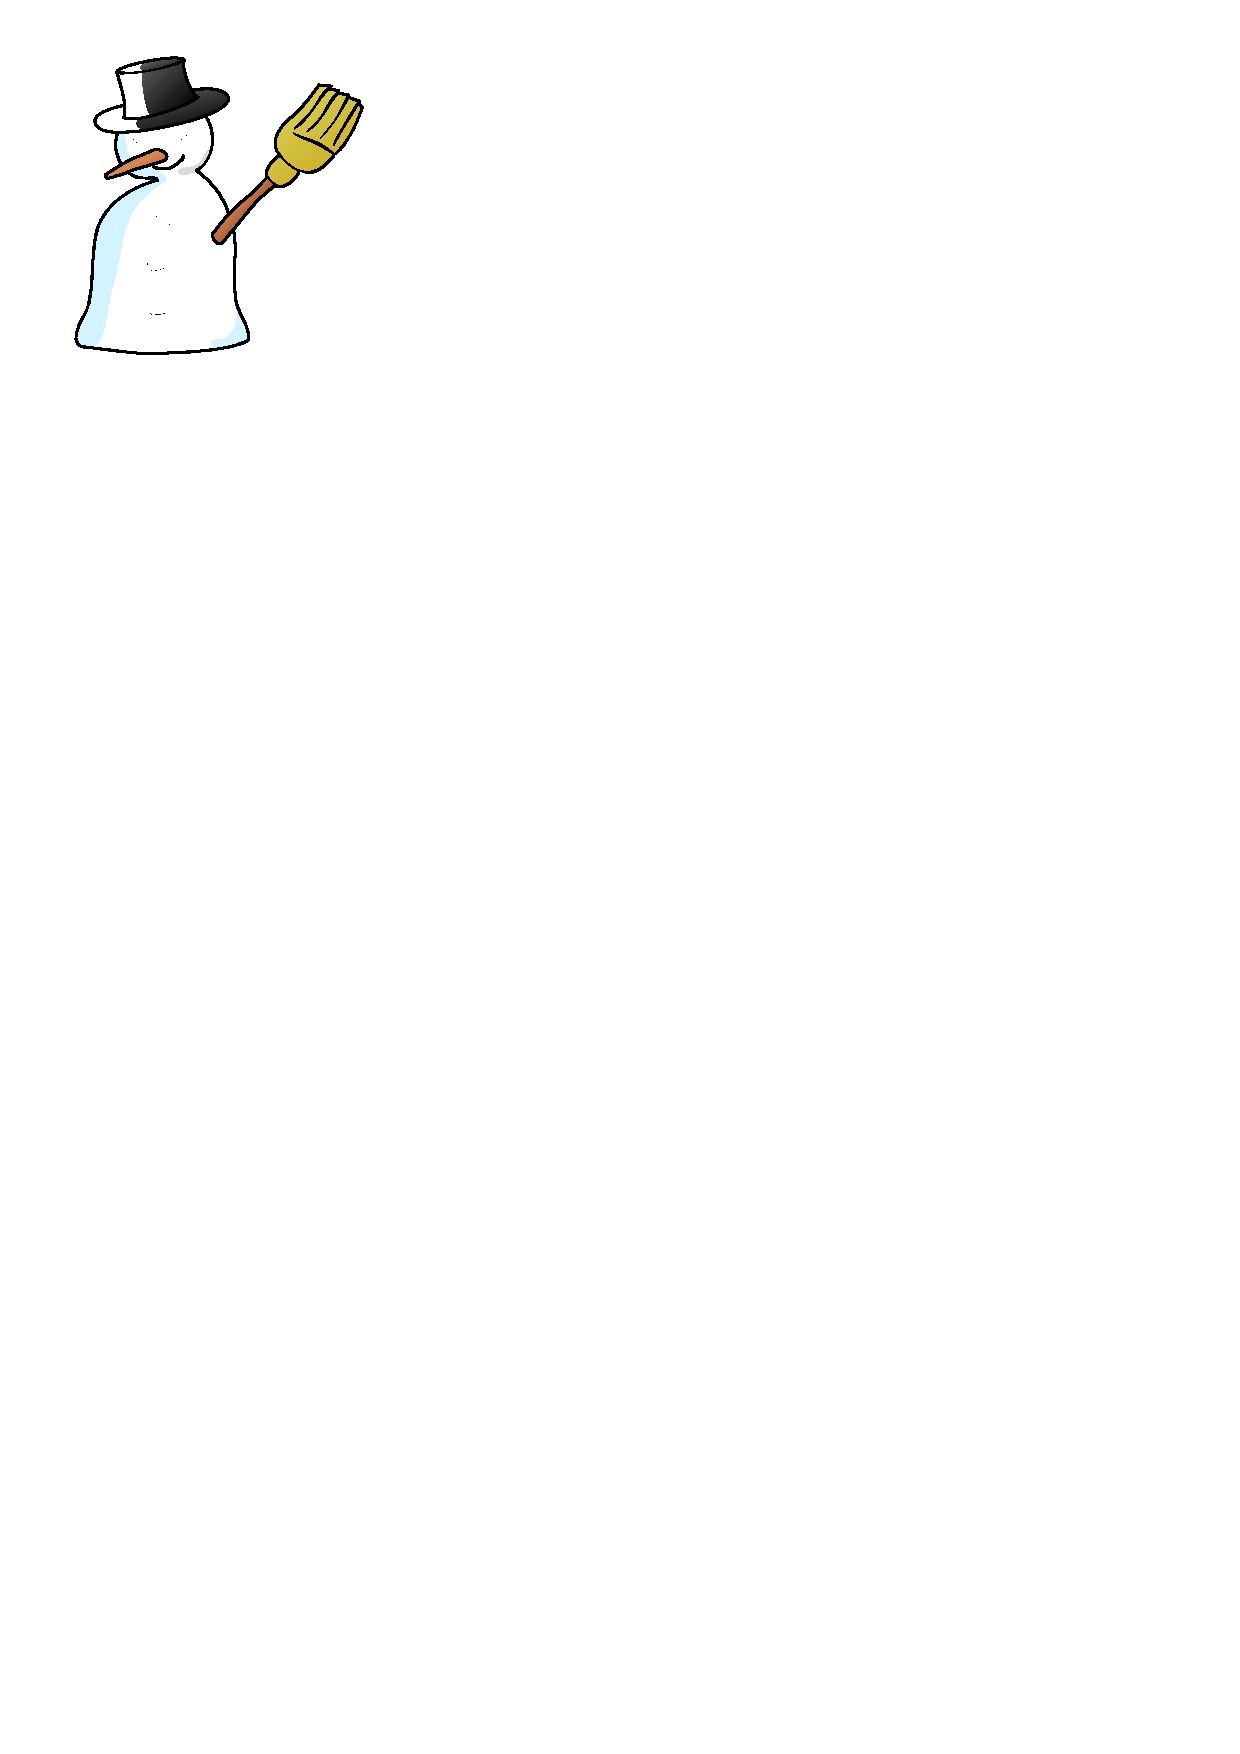
\includegraphics[width=2cm]{snowman-vectorial}
%   \caption{A snow-man}
% \end{wrapfigure}	
% 
% \noindent\verb!\usepackage{wrapfig}!\\
% This then gives you access to:\\
% \verb!\begin{wrapfigure}[lineheight]{alignment}{width}!\\
% Alignment can normally be either ``l'' for left, or ``r'' for right. Lowercase ``l'' or ``r'' forces the figure to start precisely where specified (and may cause it to run over page breaks), while capital ``L'' or ``R'' allows the figure to float. If you defined your document as twosided, the alignment can also be ``i'' for inside or ``o'' for outside, as well as ``I'' or ``O''. The width is obviously the width of the figure. The example above was introduced with:
% \lstset{language=TeX, morekeywords={\begin,\includegraphics,\caption}, caption=Wrapfig Example, label=lst:latex_example}
% \begin{lstlisting}
% 	\begin{wrapfigure}{l}{2.5cm}
% 	  \centering
% 	    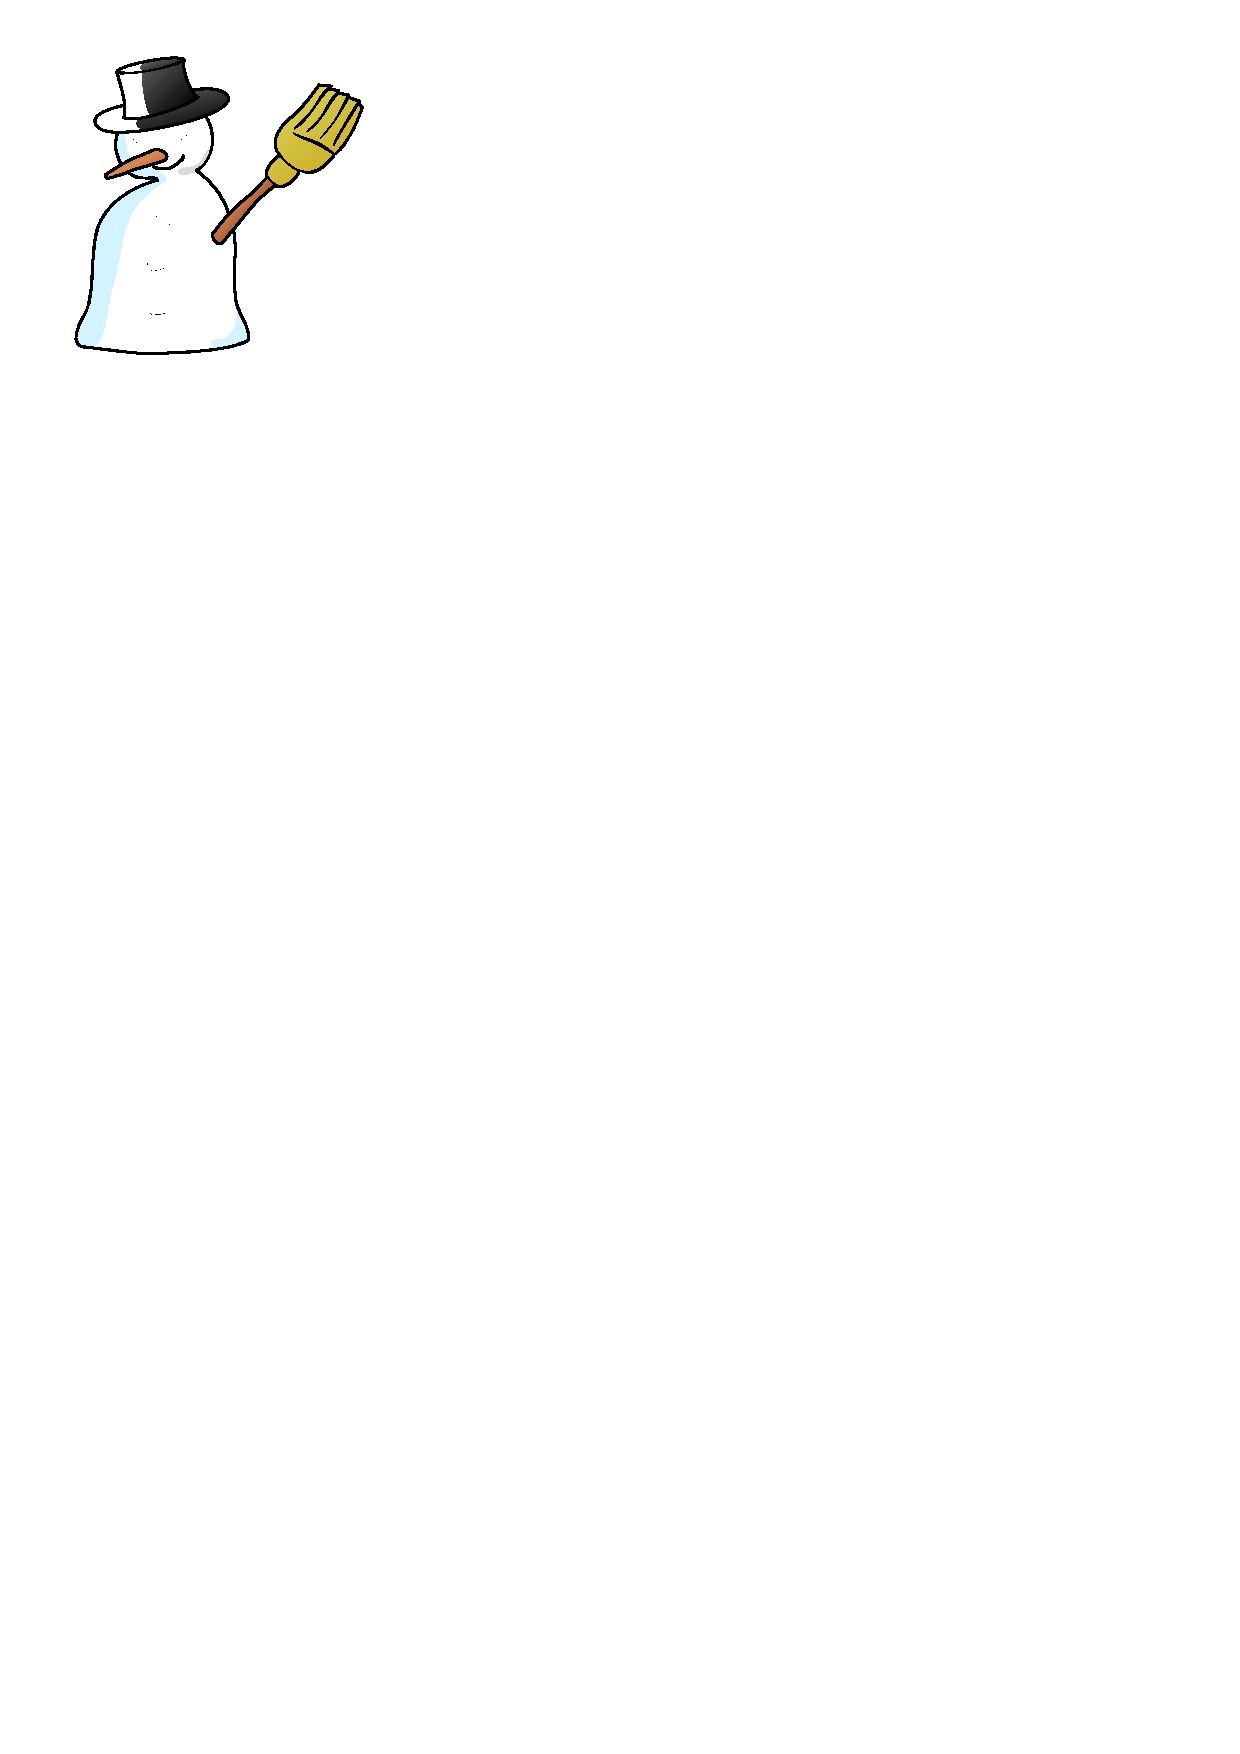
\includegraphics[width=2cm]{snowman-vectorial}
% 	  \caption{A snow-man}
% 	\end{wrapfigure}	
% \end{lstlisting}

% subsection inserting_images_wrapped_with_text (end)

% section floats_figures_and_captions (end)



%%%%%%%%%%%%%%%%%%%%%%%%%%%%%%%%%%%%%%%%%%%%%%%%%%%%%%%%%%%%%%%%%%%%
% Comments
\begin{comment}

\begin{figure}[htbp]
\centering
 \subbottom[One sub-figure]{%
    
\includegraphics[width=0.5\linewidth]{knitting-vectorial}}%
 \subbottom[Another sub-figure]{%
    
\includegraphics[width=0.5\linewidth]{knitting-vectorial}}
\caption{A figure with two sub-figures!}
\label{fig:fig2subfig}
\end{figure}






\newpage

{\Large To be included in the sections above}\\

Para fazer citações, deverá usar-se a chave da referência no ficheiro BibTeX. Se for uma única referência~\cite{Artho04}, usar um ``\verb!~!'' para ligar o \verb!\cite{...}! à palavra que o precede (\ldots\verb!referência~\cite{Artho04}!).  Caso queira fazer múltiplas citações~\cite{Shavit95,Silberschatz06,Moss85}, deverá agrupá-las dentro de um úinico \verb!\cite{...}!.

Note que o ficheiro de bibliografia pode ter tantas entradas quantas quiser. Apenas aquelas cuja chave seja referenciada no texto é que serão incluidas na listagem de bibliografia.


Footnotes\footnote{This is a simple footnote.} will be numbered and shown in the bottom of the page.


A Tabela~\ref{tab:hla:results} ilustra alguns conceitos importantes associados à contrução de tabelas:
\begin{asparaenum}[i)]
	\item Não usar linhas verticais;
	\item A legenda deve ficar por cima da tabela;
	\item Usar as macros \verb!\toprule!, \verb!\midrule! e \verb!\bottomrule! para fazer a linha horizontal superior, interiores e inferior, respectivamente.
\end{asparaenum}
 
\begin{table}[ht]
	\caption{Test results summary.}
	\label{tab:hla:results}
\centering
\begin{tabular}{lccccc}
	\toprule
	\multicolumn{1}{c}{\textbf{Test}} 	& \textbf{Anomalies}	& \textbf{Warnings}	& \textbf{Correct} 	& \textbf{Categories}		& \textbf{Missed} \\
	\midrule
\cite{Beckman08}~Connection 	& 2 & 2	& 1	& \emph{C}				& 1 \\
\cite{Artho03}~Coordinates'03 	& 1	& 4	& 1	& \emph{2B, 1C}			& 0 \\
\cite{Artho03}~Local Variable	& 1	& 2	& 1	& \emph{A}				& 0 \\
\cite{Artho03}~NASA				& 1	& 1	& 1	& ---					& 0 \\
\cite{Artho04}~Coordinates'04	& 1	& 4	& 1	& \emph{3C}				& 0 \\
\cite{Artho04}~Buffer			& 0	& 7	& 0	& \emph{2A, 1B, 2C, 2D}	& 0 \\
\cite{Artho04}~Double-Check		& 0	& 2	& 0	& \emph{1A, 1B}			& 0 \\
\cite{Flanagan04}~StringBuffer	& 1	& 0	& 0	& ---					& 1 \\
\cite{Praun03}~Account			& 1	& 1	& 1	& ---					& 0 \\
\cite{Praun03}~Jigsaw			& 1	& 2	& 1	& \emph{C}				& 0 \\
\cite{Praun03}~Over-reporting	& 0	& 2	& 0	& \emph{1A, 1C}			& 0 \\
\cite{Praun03}~Under-reporting	& 1	& 1	& 1	& ---					& 0 \\
\cite{IBM-Rep}~Allocate Vector	& 1	& 2	& 1	& \emph{C}				& 0 \\
Knight Moves					& 1	& 3	& 1	& \emph{2B}				& 0 \\
	\midrule
	\textbf{Total}			& \textbf{12}		& \textbf{33}		& \textbf{10}			& \textbf{5A, 6B, 10C, 2D}	& \textbf{2} \\
	\bottomrule
\end{tabular}
\end{table}



\begin{figure}[htbp]
	\centering
    \subbottom[Novelo de lã] {%
		\label{fig:novelo}
		
\includegraphics[height=1in]{knitting-vectorial}
    }
\qquad\qquad
    \subbottom[Tempestade com neve] {%
		\label{fig:nuvem}
		
\includegraphics[height=1in]{snowstorm-vectorial}
    }
  \caption{Exemplo de utilização de \emph{subbottom}}
  \label{fig:figura-completa}
\end{figure}


Para incluir listagens de código no seu documento, deverá incluir o pacote \emph{listings} e depois usar o ambiente \emph{lstlisting}, como exemplificado na Listagem~\ref{lst:HelloWorld}.

\lstset{language=Java, caption=Hello World, label=lst:HelloWorld}
\begin{lstlisting}
/** 
 * The HelloWorldApp class implements an application that
 * simply prints "Hello World!" to standard output.
 */
class HelloWorldApp {%
    public static void main(String[] args) {%
        System.out.println("Hello World!"); // Display the string.
    }
}
\end{lstlisting}


\end{comment}